\documentclass[]{article}
\usepackage{lmodern}
\usepackage{amssymb,amsmath}
\usepackage{ifxetex,ifluatex}
\usepackage{fixltx2e} % provides \textsubscript
\ifnum 0\ifxetex 1\fi\ifluatex 1\fi=0 % if pdftex
  \usepackage[T1]{fontenc}
  \usepackage[utf8]{inputenc}
\else % if luatex or xelatex
  \ifxetex
    \usepackage{mathspec}
  \else
    \usepackage{fontspec}
  \fi
  \defaultfontfeatures{Ligatures=TeX,Scale=MatchLowercase}
\fi
% use upquote if available, for straight quotes in verbatim environments
\IfFileExists{upquote.sty}{\usepackage{upquote}}{}
% use microtype if available
\IfFileExists{microtype.sty}{%
\usepackage{microtype}
\UseMicrotypeSet[protrusion]{basicmath} % disable protrusion for tt fonts
}{}
\usepackage[margin=1in]{geometry}
\usepackage{hyperref}
\PassOptionsToPackage{usenames,dvipsnames}{color} % color is loaded by hyperref
\hypersetup{unicode=true,
            pdftitle={Simple Markdown Example},
            pdfauthor={Jenny Rieck; Derek Beaton},
            colorlinks=true,
            linkcolor=Maroon,
            citecolor=Blue,
            urlcolor=blue,
            breaklinks=true}
\urlstyle{same}  % don't use monospace font for urls
\usepackage{color}
\usepackage{fancyvrb}
\newcommand{\VerbBar}{|}
\newcommand{\VERB}{\Verb[commandchars=\\\{\}]}
\DefineVerbatimEnvironment{Highlighting}{Verbatim}{commandchars=\\\{\}}
% Add ',fontsize=\small' for more characters per line
\usepackage{framed}
\definecolor{shadecolor}{RGB}{248,248,248}
\newenvironment{Shaded}{\begin{snugshade}}{\end{snugshade}}
\newcommand{\AlertTok}[1]{\textcolor[rgb]{0.94,0.16,0.16}{#1}}
\newcommand{\AnnotationTok}[1]{\textcolor[rgb]{0.56,0.35,0.01}{\textbf{\textit{#1}}}}
\newcommand{\AttributeTok}[1]{\textcolor[rgb]{0.77,0.63,0.00}{#1}}
\newcommand{\BaseNTok}[1]{\textcolor[rgb]{0.00,0.00,0.81}{#1}}
\newcommand{\BuiltInTok}[1]{#1}
\newcommand{\CharTok}[1]{\textcolor[rgb]{0.31,0.60,0.02}{#1}}
\newcommand{\CommentTok}[1]{\textcolor[rgb]{0.56,0.35,0.01}{\textit{#1}}}
\newcommand{\CommentVarTok}[1]{\textcolor[rgb]{0.56,0.35,0.01}{\textbf{\textit{#1}}}}
\newcommand{\ConstantTok}[1]{\textcolor[rgb]{0.00,0.00,0.00}{#1}}
\newcommand{\ControlFlowTok}[1]{\textcolor[rgb]{0.13,0.29,0.53}{\textbf{#1}}}
\newcommand{\DataTypeTok}[1]{\textcolor[rgb]{0.13,0.29,0.53}{#1}}
\newcommand{\DecValTok}[1]{\textcolor[rgb]{0.00,0.00,0.81}{#1}}
\newcommand{\DocumentationTok}[1]{\textcolor[rgb]{0.56,0.35,0.01}{\textbf{\textit{#1}}}}
\newcommand{\ErrorTok}[1]{\textcolor[rgb]{0.64,0.00,0.00}{\textbf{#1}}}
\newcommand{\ExtensionTok}[1]{#1}
\newcommand{\FloatTok}[1]{\textcolor[rgb]{0.00,0.00,0.81}{#1}}
\newcommand{\FunctionTok}[1]{\textcolor[rgb]{0.00,0.00,0.00}{#1}}
\newcommand{\ImportTok}[1]{#1}
\newcommand{\InformationTok}[1]{\textcolor[rgb]{0.56,0.35,0.01}{\textbf{\textit{#1}}}}
\newcommand{\KeywordTok}[1]{\textcolor[rgb]{0.13,0.29,0.53}{\textbf{#1}}}
\newcommand{\NormalTok}[1]{#1}
\newcommand{\OperatorTok}[1]{\textcolor[rgb]{0.81,0.36,0.00}{\textbf{#1}}}
\newcommand{\OtherTok}[1]{\textcolor[rgb]{0.56,0.35,0.01}{#1}}
\newcommand{\PreprocessorTok}[1]{\textcolor[rgb]{0.56,0.35,0.01}{\textit{#1}}}
\newcommand{\RegionMarkerTok}[1]{#1}
\newcommand{\SpecialCharTok}[1]{\textcolor[rgb]{0.00,0.00,0.00}{#1}}
\newcommand{\SpecialStringTok}[1]{\textcolor[rgb]{0.31,0.60,0.02}{#1}}
\newcommand{\StringTok}[1]{\textcolor[rgb]{0.31,0.60,0.02}{#1}}
\newcommand{\VariableTok}[1]{\textcolor[rgb]{0.00,0.00,0.00}{#1}}
\newcommand{\VerbatimStringTok}[1]{\textcolor[rgb]{0.31,0.60,0.02}{#1}}
\newcommand{\WarningTok}[1]{\textcolor[rgb]{0.56,0.35,0.01}{\textbf{\textit{#1}}}}
\usepackage{graphicx,grffile}
\makeatletter
\def\maxwidth{\ifdim\Gin@nat@width>\linewidth\linewidth\else\Gin@nat@width\fi}
\def\maxheight{\ifdim\Gin@nat@height>\textheight\textheight\else\Gin@nat@height\fi}
\makeatother
% Scale images if necessary, so that they will not overflow the page
% margins by default, and it is still possible to overwrite the defaults
% using explicit options in \includegraphics[width, height, ...]{}
\setkeys{Gin}{width=\maxwidth,height=\maxheight,keepaspectratio}
\IfFileExists{parskip.sty}{%
\usepackage{parskip}
}{% else
\setlength{\parindent}{0pt}
\setlength{\parskip}{6pt plus 2pt minus 1pt}
}
\setlength{\emergencystretch}{3em}  % prevent overfull lines
\providecommand{\tightlist}{%
  \setlength{\itemsep}{0pt}\setlength{\parskip}{0pt}}
\setcounter{secnumdepth}{0}
% Redefines (sub)paragraphs to behave more like sections
\ifx\paragraph\undefined\else
\let\oldparagraph\paragraph
\renewcommand{\paragraph}[1]{\oldparagraph{#1}\mbox{}}
\fi
\ifx\subparagraph\undefined\else
\let\oldsubparagraph\subparagraph
\renewcommand{\subparagraph}[1]{\oldsubparagraph{#1}\mbox{}}
\fi

%%% Use protect on footnotes to avoid problems with footnotes in titles
\let\rmarkdownfootnote\footnote%
\def\footnote{\protect\rmarkdownfootnote}

%%% Change title format to be more compact
\usepackage{titling}

% Create subtitle command for use in maketitle
\newcommand{\subtitle}[1]{
  \posttitle{
    \begin{center}\large#1\end{center}
    }
}

\setlength{\droptitle}{-2em}

  \title{Simple Markdown Example}
    \pretitle{\vspace{\droptitle}\centering\huge}
  \posttitle{\par}
  \subtitle{PDF/LaTex version}
  \author{Jenny Rieck \\ Derek Beaton}
    \preauthor{\centering\large\emph}
  \postauthor{\par}
      \predate{\centering\large\emph}
  \postdate{\par}
    \date{May 13, 2019}

\usepackage{booktabs}
\usepackage{longtable}
\usepackage{array}
\usepackage{multirow}
\usepackage[table]{xcolor}
\usepackage{wrapfig}
\usepackage{float}
\usepackage{colortbl}
\usepackage{pdflscape}
\usepackage{tabu}
\usepackage{threeparttable}
\usepackage{threeparttablex}
\usepackage[normalem]{ulem}
\usepackage{makecell}

\begin{document}
\maketitle

\hypertarget{introduction}{%
\section{Introduction}\label{introduction}}

For reference, see
\href{https://emilyriederer.netlify.com/post/rmarkdown-driven-development/}{RMarkdown
Driven Development} by Emily Riederer for a comprehensive overview of
how to best structure RMarkdown for projects, packages, and other
development-driven tasks.

In general for this RMarkdown file we follow Emily's fourth example with
a directory structure, minimized redundancies, and heavy-duty code
elsewhere. This RMarkdown, generally, serves as place to describe,
analyze, and visualize our data. Thus, this text is shown at the top of
the output, but actually appears after several \texttt{R} code chunks,
which exist between the \texttt{Introduction} heading and YAML header
information (which you see as title, authors, dates, etc\ldots{}).

Most of the RMarkdown files in this directory will show generally the
same content, but help highlight the different ways you can use
RMarkdown, \texttt{knitr}, \texttt{pandoc}, \texttt{LateX}, and various
package built for those, such as \texttt{beamer} (\texttt{LateX}) for
presentations, and
\href{https://github.com/crsh/papaja}{\texttt{papaja}} \&
\href{https://github.com/rstudio/rticles}{\texttt{rticles}}
(R/RMarkdown) for writing manuscripts that export to \texttt{LaTeX} or
MS Word. If you decide to write MS Word documents through RMarkdown, you
should also use the
\href{https://github.com/noamross/redoc}{\texttt{redoc} package}.

\hypertarget{r-chunks-a-word-of-caution}{%
\subsection{R chunks: A word of
caution}\label{r-chunks-a-word-of-caution}}

It is good practice to name your \texttt{R} chunks. If you do not, then
the \texttt{R} chunks will still produce the intended material. However,
when you do name them, you should ensure they have unique names (else,
you will likely see some cryptic and not always informative error
messages).

\hypertarget{tables}{%
\section{Tables}\label{tables}}

There are multiple approaches and packages to help visualize tables or
tabular information. Let's start by looking at a simple summary of all
the continuous variables. First, we will visualize the summary table
through two methods within R: \texttt{knitr::kable} and the
\texttt{kablExtra} package, followed by \texttt{grid} and
\texttt{gridExtra}. Next, we will use the same data and illustrate what
happens when we pass it to Python through \texttt{reticulate}.

In this section we wil also show the code chunks that generate these
tables and visuals, which are embedded in the RMarkdown document.

\hypertarget{knitr-and-kableextra}{%
\subsection{knitr and kableExtra}\label{knitr-and-kableextra}}

To make HTML and LaTeX tables in RMarkdown, one of the easiest and most
common options is through \texttt{knitr}. The \texttt{knitr} package is,
effectively, the tool to make RMarkdown documents go from R \& RMarkdown
(plus other code and LaTeX) into PDFs or HTML pages. We'll start with
the \texttt{knitr::kable()}.

\begin{Shaded}
\begin{Highlighting}[]
\NormalTok{example_table <-}\StringTok{ }\NormalTok{amerge_subset[, }\KeywordTok{c}\NormalTok{(}\StringTok{"AGE"}\NormalTok{, }\StringTok{"MOCA"}\NormalTok{, }\StringTok{"CDRSB"}\NormalTok{, }\StringTok{"WholeBrain"}\NormalTok{, }
    \StringTok{"Hippocampus"}\NormalTok{, }\StringTok{"MidTemp"}\NormalTok{)]}
\NormalTok{example_table_Dx <-}\StringTok{ }\NormalTok{amerge_subset[, }\KeywordTok{c}\NormalTok{(}\StringTok{"DX"}\NormalTok{, }\StringTok{"AGE"}\NormalTok{, }\StringTok{"MOCA"}\NormalTok{, }\StringTok{"CDRSB"}\NormalTok{, }
    \StringTok{"WholeBrain"}\NormalTok{, }\StringTok{"Hippocampus"}\NormalTok{, }\StringTok{"MidTemp"}\NormalTok{)]}
\end{Highlighting}
\end{Shaded}

\begin{Shaded}
\begin{Highlighting}[]
\KeywordTok{kable}\NormalTok{(}\KeywordTok{summary}\NormalTok{(example_table))}
\end{Highlighting}
\end{Shaded}

\begin{tabular}{l|l|l|l|l|l|l}
\hline
  &      AGE &      MOCA &     CDRSB &   WholeBrain &  Hippocampus &    MidTemp\\
\hline
 & Min.   :55.00 & Min.   :16.00 & Min.   :0.000 & Min.   : 817421 & Min.   : 3731 & Min.   :12213\\
\hline
 & 1st Qu.:67.20 & 1st Qu.:22.00 & 1st Qu.:0.000 & 1st Qu.: 984410 & 1st Qu.: 6510 & 1st Qu.:18535\\
\hline
 & Median :71.90 & Median :24.00 & Median :1.000 & Median :1051621 & Median : 7223 & Median :20186\\
\hline
 & Mean   :71.92 & Mean   :23.89 & Mean   :1.202 & Mean   :1057026 & Mean   : 7150 & Mean   :20302\\
\hline
 & 3rd Qu.:76.60 & 3rd Qu.:26.00 & 3rd Qu.:2.000 & 3rd Qu.:1120570 & 3rd Qu.: 7834 & 3rd Qu.:22088\\
\hline
 & Max.   :89.60 & Max.   :30.00 & Max.   :5.500 & Max.   :1486036 & Max.   :10602 & Max.   :32189\\
\hline
\end{tabular}

But that is not particularly nice looking. So we can use some parameters
to make this table look better (which depend on having LaTeX).

\begin{Shaded}
\begin{Highlighting}[]
\KeywordTok{kable}\NormalTok{(}\KeywordTok{summary}\NormalTok{(example_table), }\DataTypeTok{format =} \StringTok{"latex"}\NormalTok{, }\DataTypeTok{booktabs =}\NormalTok{ T)}
\end{Highlighting}
\end{Shaded}

\begin{tabular}{lllllll}
\toprule
  &      AGE &      MOCA &     CDRSB &   WholeBrain &  Hippocampus &    MidTemp\\
\midrule
 & Min.   :55.00 & Min.   :16.00 & Min.   :0.000 & Min.   : 817421 & Min.   : 3731 & Min.   :12213\\
 & 1st Qu.:67.20 & 1st Qu.:22.00 & 1st Qu.:0.000 & 1st Qu.: 984410 & 1st Qu.: 6510 & 1st Qu.:18535\\
 & Median :71.90 & Median :24.00 & Median :1.000 & Median :1051621 & Median : 7223 & Median :20186\\
 & Mean   :71.92 & Mean   :23.89 & Mean   :1.202 & Mean   :1057026 & Mean   : 7150 & Mean   :20302\\
 & 3rd Qu.:76.60 & 3rd Qu.:26.00 & 3rd Qu.:2.000 & 3rd Qu.:1120570 & 3rd Qu.: 7834 & 3rd Qu.:22088\\
 & Max.   :89.60 & Max.   :30.00 & Max.   :5.500 & Max.   :1486036 & Max.   :10602 & Max.   :32189\\
\bottomrule
\end{tabular}

With \texttt{booktabs} and \texttt{latex} format, we've made the table
look a little better. But can we make it look even better than that? We
can with \texttt{kableExtra}.

\begin{Shaded}
\begin{Highlighting}[]
\KeywordTok{kable}\NormalTok{(}\KeywordTok{summary}\NormalTok{(example_table), }\DataTypeTok{format =} \StringTok{"latex"}\NormalTok{, }\DataTypeTok{booktabs =}\NormalTok{ T) }\OperatorTok\StringTok{ }
\StringTok{    }\KeywordTok{kable_styling}\NormalTok{(}\DataTypeTok{font_size =} \DecValTok{10}\NormalTok{, }\DataTypeTok{position =} \StringTok{"center"}\NormalTok{)}
\end{Highlighting}
\end{Shaded}

\begin{table}[H]
\centering\begingroup\fontsize{10}{12}\selectfont

\begin{tabular}{lllllll}
\toprule
  &      AGE &      MOCA &     CDRSB &   WholeBrain &  Hippocampus &    MidTemp\\
\midrule
 & Min.   :55.00 & Min.   :16.00 & Min.   :0.000 & Min.   : 817421 & Min.   : 3731 & Min.   :12213\\
 & 1st Qu.:67.20 & 1st Qu.:22.00 & 1st Qu.:0.000 & 1st Qu.: 984410 & 1st Qu.: 6510 & 1st Qu.:18535\\
 & Median :71.90 & Median :24.00 & Median :1.000 & Median :1051621 & Median : 7223 & Median :20186\\
 & Mean   :71.92 & Mean   :23.89 & Mean   :1.202 & Mean   :1057026 & Mean   : 7150 & Mean   :20302\\
 & 3rd Qu.:76.60 & 3rd Qu.:26.00 & 3rd Qu.:2.000 & 3rd Qu.:1120570 & 3rd Qu.: 7834 & 3rd Qu.:22088\\
 & Max.   :89.60 & Max.   :30.00 & Max.   :5.500 & Max.   :1486036 & Max.   :10602 & Max.   :32189\\
\bottomrule
\end{tabular}\endgroup{}
\end{table}

We can take the table look even further with additional options, like
``stripes''.

\begin{Shaded}
\begin{Highlighting}[]
\KeywordTok{kable}\NormalTok{(}\KeywordTok{summary}\NormalTok{(example_table), }\DataTypeTok{format =} \StringTok{"latex"}\NormalTok{, }\DataTypeTok{booktabs =}\NormalTok{ T) }\OperatorTok\StringTok{ }
\StringTok{    }\KeywordTok{kable_styling}\NormalTok{(}\DataTypeTok{font_size =} \DecValTok{10}\NormalTok{, }\DataTypeTok{position =} \StringTok{"center"}\NormalTok{, }\DataTypeTok{latex_options =} \StringTok{"striped"}\NormalTok{)}
\end{Highlighting}
\end{Shaded}

\begin{table}[H]
\centering\begingroup\fontsize{10}{12}\selectfont
\rowcolors{2}{gray!6}{white}

\begin{tabular}{lllllll}
\hiderowcolors
\toprule
  &      AGE &      MOCA &     CDRSB &   WholeBrain &  Hippocampus &    MidTemp\\
\midrule
\showrowcolors
 & Min.   :55.00 & Min.   :16.00 & Min.   :0.000 & Min.   : 817421 & Min.   : 3731 & Min.   :12213\\
 & 1st Qu.:67.20 & 1st Qu.:22.00 & 1st Qu.:0.000 & 1st Qu.: 984410 & 1st Qu.: 6510 & 1st Qu.:18535\\
 & Median :71.90 & Median :24.00 & Median :1.000 & Median :1051621 & Median : 7223 & Median :20186\\
 & Mean   :71.92 & Mean   :23.89 & Mean   :1.202 & Mean   :1057026 & Mean   : 7150 & Mean   :20302\\
 & 3rd Qu.:76.60 & 3rd Qu.:26.00 & 3rd Qu.:2.000 & 3rd Qu.:1120570 & 3rd Qu.: 7834 & 3rd Qu.:22088\\
 & Max.   :89.60 & Max.   :30.00 & Max.   :5.500 & Max.   :1486036 & Max.   :10602 & Max.   :32189\\
\bottomrule
\end{tabular}
\rowcolors{2}{white}{white}\endgroup{}
\end{table}

Given that we have redundant information in the table (min/max,
etc\ldots{}) we can do a better job and make an even nicer table with an
\texttt{apply()}, and then use multiple \texttt{kable} and
\texttt{kableExtra} features to make a really nice table.

\begin{Shaded}
\begin{Highlighting}[]
\NormalTok{better_example_table <-}\StringTok{ }\KeywordTok{apply}\NormalTok{(example_table, }\DecValTok{2}\NormalTok{, summary)}

\KeywordTok{kable}\NormalTok{(better_example_table, }\DataTypeTok{format =} \StringTok{"latex"}\NormalTok{, }\DataTypeTok{booktabs =}\NormalTok{ T, }\DataTypeTok{digits =} \DecValTok{2}\NormalTok{) }\OperatorTok\StringTok{ }
\StringTok{    }\NormalTok{kableExtra}\OperatorTok{::}\KeywordTok{add_header_above}\NormalTok{(}\KeywordTok{c}\NormalTok{(}\DataTypeTok{Statistic =} \DecValTok{1}\NormalTok{, }\DataTypeTok{Demographic =} \DecValTok{1}\NormalTok{, }
        \DataTypeTok{Clinical =} \DecValTok{2}\NormalTok{, }\DataTypeTok{Brain =} \DecValTok{3}\NormalTok{)) }\OperatorTok\StringTok{ }\KeywordTok{kable_styling}\NormalTok{(}\DataTypeTok{font_size =} \DecValTok{10}\NormalTok{, }
    \DataTypeTok{position =} \StringTok{"center"}\NormalTok{, }\DataTypeTok{latex_options =} \StringTok{"striped"}\NormalTok{) }\OperatorTok\StringTok{ }\KeywordTok{row_spec}\NormalTok{(}\DecValTok{0}\NormalTok{, }
    \DataTypeTok{angle =} \DecValTok{15}\NormalTok{, }\DataTypeTok{bold =}\NormalTok{ T)}
\end{Highlighting}
\end{Shaded}

\begin{table}[H]
\centering\begingroup\fontsize{10}{12}\selectfont
\rowcolors{2}{gray!6}{white}

\begin{tabular}{lrrrrrr}
\hiderowcolors
\toprule
\multicolumn{1}{c}{Statistic} & \multicolumn{1}{c}{Demographic} & \multicolumn{2}{c}{Clinical} & \multicolumn{3}{c}{Brain} \\
\cmidrule(l{2pt}r{2pt}){1-1} \cmidrule(l{2pt}r{2pt}){2-2} \cmidrule(l{2pt}r{2pt}){3-4} \cmidrule(l{2pt}r{2pt}){5-7}
\rotatebox{15}{\textbf{ }} & \rotatebox{15}{\textbf{AGE}} & \rotatebox{15}{\textbf{MOCA}} & \rotatebox{15}{\textbf{CDRSB}} & \rotatebox{15}{\textbf{WholeBrain}} & \rotatebox{15}{\textbf{Hippocampus}} & \rotatebox{15}{\textbf{MidTemp}}\\
\midrule
\showrowcolors
Min. & 55.00 & 16.00 & 0.0 & 817421.2 & 3731.00 & 12213.00\\
1st Qu. & 67.20 & 22.00 & 0.0 & 984409.9 & 6510.00 & 18535.00\\
Median & 71.90 & 24.00 & 1.0 & 1051621.3 & 7223.00 & 20186.00\\
Mean & 71.92 & 23.89 & 1.2 & 1057025.6 & 7149.61 & 20301.93\\
3rd Qu. & 76.60 & 26.00 & 2.0 & 1120569.5 & 7834.00 & 22088.00\\
Max. & 89.60 & 30.00 & 5.5 & 1486035.6 & 10602.00 & 32189.00\\
\bottomrule
\end{tabular}
\rowcolors{2}{white}{white}\endgroup{}
\end{table}

\hypertarget{grid-and-gridextra}{%
\subsection{grid and gridExtra}\label{grid-and-gridextra}}

Sometimes we need tables to be graphics. This is where the \texttt{grid}
and \texttt{gridExtra} packages come in. The \texttt{grid} package uses
\texttt{grob}s to turn items---tables, figures, all sorts of
things---into configurable parts of a figure.

\begin{Shaded}
\begin{Highlighting}[]
\KeywordTok{grid.table}\NormalTok{(better_example_table)}
\end{Highlighting}
\end{Shaded}

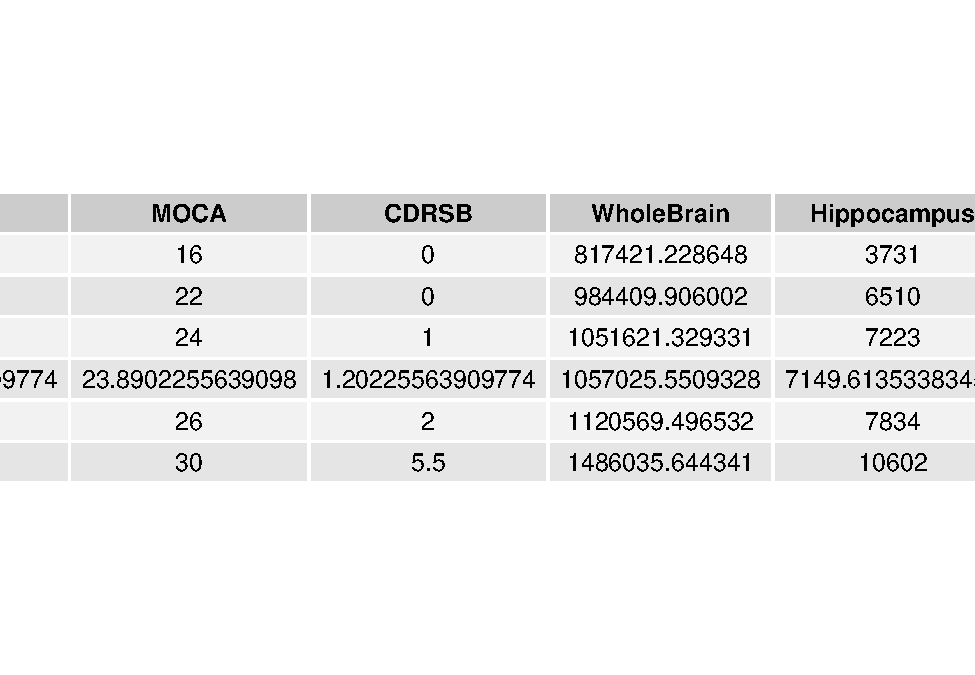
\includegraphics{1_a_Simple_RMarkdown_PDF_files/figure-latex/grid_and_gridExtra-1.pdf}

But it's clear we have a few extra things we should do to make this
figure of a table look better.

\begin{Shaded}
\begin{Highlighting}[]
\NormalTok{better_example_table_round <-}\StringTok{ }\KeywordTok{apply}\NormalTok{(better_example_table, }\DecValTok{2}\NormalTok{, }
\NormalTok{    format, }\DataTypeTok{digits =} \DecValTok{2}\NormalTok{, }\DataTypeTok{nsmall =} \DecValTok{2}\NormalTok{)}

\KeywordTok{grid.table}\NormalTok{(better_example_table_round)}
\end{Highlighting}
\end{Shaded}

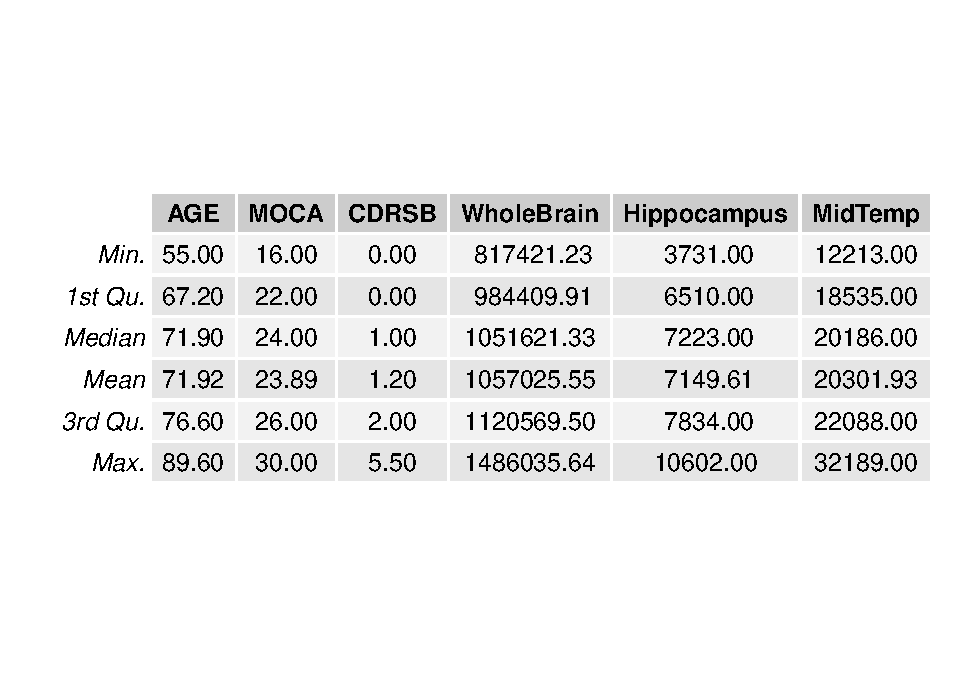
\includegraphics{1_a_Simple_RMarkdown_PDF_files/figure-latex/grid_and_gridExtra_round-1.pdf}

However, the \texttt{grid} and \texttt{gridExtra} packages can be
difficult to customize many of the pieces. Therefore it might be easier
to stick to the \texttt{LaTeX} approaches with \texttt{kable} or it is
well worth checking out the
\href{https://github.com/rstudio/gt}{\texttt{gt} package}.

\hypertarget{python-via-reticulate}{%
\subsection{Python via reticulate}\label{python-via-reticulate}}

What if you now love RMarkdown but are still really into Python? Not a
problem. The
\href{https://rstudio.github.io/reticulate/}{\texttt{reticulate}
package} has you covered. It's an R package to connect to your
\texttt{Python} installation and bring the data or results back into
\texttt{R}, but with some of the same features as you're used to in
either \texttt{Python} or \texttt{R}. Let's start out with a \emph{head
to head} of \texttt{R}'s \texttt{head()} vs.~\texttt{Python}'s
\texttt{.head()}.

In \texttt{R} we write the call in RMarkdown as if we would normally in
\texttt{R}:

\begin{Shaded}
\begin{Highlighting}[]
\KeywordTok{head}\NormalTok{(example_table)}
\end{Highlighting}
\end{Shaded}

\begin{verbatim}
##       AGE MOCA CDRSB WholeBrain Hippocampus MidTemp
## 2002 64.8   28   2.5  1135556.6        7960   21867
## 2003 63.6   24   2.0  1070369.5        7611   21580
## 2007 83.4   23   2.5   920710.1        5614   20567
## 2010 62.9   27   0.5   986402.9        8004   20358
## 2011 69.9   25   1.5   987822.5        6686   20366
## 2018 76.4   26   1.5  1004817.0        7774   19531
\end{verbatim}

Unlike the previous code chunks, we have to tell RMarkdown that the
language it should expect is \texttt{python} instead of \texttt{R}.

\begin{Shaded}
\begin{Highlighting}[]
\BuiltInTok{print}\NormalTok{(r.example_table.head())}
\end{Highlighting}
\end{Shaded}

\begin{verbatim}
##        AGE  MOCA  CDRSB    WholeBrain  Hippocampus  MidTemp
## 2002  64.8  28.0    2.5  1.135557e+06       7960.0  21867.0
## 2003  63.6  24.0    2.0  1.070369e+06       7611.0  21580.0
## 2007  83.4  23.0    2.5  9.207101e+05       5614.0  20567.0
## 2010  62.9  27.0    0.5  9.864029e+05       8004.0  20358.0
## 2011  69.9  25.0    1.5  9.878225e+05       6686.0  20366.0
\end{verbatim}

For \texttt{Python} via \texttt{R} we also need to use the \texttt{.}
(dot notation) because of \texttt{Python}'s object oriented approach.
From the \texttt{r} object, we get the \texttt{example\_table} attribute
and then perform the \texttt{head} method. That's because
\texttt{Python} needs to know about the object coming from \texttt{R}.

\hypertarget{here-be-.dragons}{%
\subsubsection{Here be .dragons}\label{here-be-.dragons}}

For those more familiar with \texttt{R} style that stems from the
\href{}{\texttt{S} language origin} or \href{}{Google's style guide},
the \texttt{.} can be a substantial source of confusion both here and in
the \texttt{tidyverse}. In base \texttt{R}, it is a valid character for
user defined items. But in base \texttt{R} it is \emph{also} used for
objects and classes (see, e.g., \texttt{.print()}). In the
\texttt{tidyverse} the \texttt{.} has a special purpose when alone (not
amongst other characters), often as a placeholder for where to pass a
variable as an argument into a function.

In \texttt{R}: use \texttt{.} either with caution or reckless abandon.

\hypertarget{passsssing-back-and-forth}{%
\subsubsection{Passsssing back and
foRth}\label{passsssing-back-and-forth}}

That subtitle is a stretch! With the \texttt{reticulate} package and
\texttt{R} we can pass items between the the two languages/environments.
And, depending on which language, we use that language's
preferred/standard approach of referring to attributes or objects. In
this next example we call into the \texttt{.describe()} method in
\texttt{Python}, which is similar to \texttt{R}'s \texttt{summary()},
but allows/requires us to define certain parameters.

\begin{Shaded}
\begin{Highlighting}[]
\NormalTok{perc }\OperatorTok{=}\NormalTok{ [.}\DecValTok{25}\NormalTok{, }\FloatTok{.50}\NormalTok{, }\FloatTok{.75}\NormalTok{] }
\NormalTok{desc }\OperatorTok{=}\NormalTok{ r.example_table.describe(percentiles }\OperatorTok{=}\NormalTok{ perc)}
\BuiltInTok{print}\NormalTok{(desc)}
\end{Highlighting}
\end{Shaded}

\begin{verbatim}
##               AGE        MOCA       CDRSB    WholeBrain   Hippocampus  \
## count  665.000000  665.000000  665.000000  6.650000e+02    665.000000   
## mean    71.922556   23.890226    1.202256  1.057026e+06   7149.613534   
## std      6.868621    3.279405    1.343238  1.036727e+05   1086.040463   
## min     55.000000   16.000000    0.000000  8.174212e+05   3731.000000   
## 25%     67.200000   22.000000    0.000000  9.844099e+05   6510.000000   
## 50%     71.900000   24.000000    1.000000  1.051621e+06   7223.000000   
## 75%     76.600000   26.000000    2.000000  1.120569e+06   7834.000000   
## max     89.600000   30.000000    5.500000  1.486036e+06  10602.000000   
## 
##             MidTemp  
## count    665.000000  
## mean   20301.933835  
## std     2675.571327  
## min    12213.000000  
## 25%    18535.000000  
## 50%    20186.000000  
## 75%    22088.000000  
## max    32189.000000
\end{verbatim}

We can visualize the results directly using the \texttt{print()} method.
But like previous results shown in \texttt{R}, we can do a lot better.
We can pass the \texttt{desc} object back to \texttt{R} with the
\texttt{\$} notation (generally for lists or simple classes in
\texttt{R}). When we retrieve an object from python (via \texttt{py\$}),
we can then do what we would usually do in \texttt{R}. Here, we go back
to \texttt{kable()} and \texttt{kable\_styling()} with some of the
parameters to make very nice looking \texttt{LaTeX} tables.

\begin{Shaded}
\begin{Highlighting}[]
\KeywordTok{kable}\NormalTok{(py}\OperatorTok{$}\NormalTok{desc, }\DataTypeTok{digits =} \DecValTok{2}\NormalTok{, }\DataTypeTok{format =} \StringTok{"latex"}\NormalTok{, }\DataTypeTok{booktabs =}\NormalTok{ T) }\OperatorTok\StringTok{ }
\StringTok{    }\KeywordTok{kable_styling}\NormalTok{(}\DataTypeTok{font_size =} \DecValTok{10}\NormalTok{, }\DataTypeTok{position =} \StringTok{"center"}\NormalTok{, }\DataTypeTok{latex_options =} \StringTok{"striped"}\NormalTok{)}
\end{Highlighting}
\end{Shaded}

\begin{table}[H]
\centering\begingroup\fontsize{10}{12}\selectfont
\rowcolors{2}{gray!6}{white}

\begin{tabular}{lrrrrrr}
\hiderowcolors
\toprule
  & AGE & MOCA & CDRSB & WholeBrain & Hippocampus & MidTemp\\
\midrule
\showrowcolors
count & 665.00 & 665.00 & 665.00 & 665.0 & 665.00 & 665.00\\
mean & 71.92 & 23.89 & 1.20 & 1057025.6 & 7149.61 & 20301.93\\
std & 6.87 & 3.28 & 1.34 & 103672.7 & 1086.04 & 2675.57\\
min & 55.00 & 16.00 & 0.00 & 817421.2 & 3731.00 & 12213.00\\
25\% & 67.20 & 22.00 & 0.00 & 984409.9 & 6510.00 & 18535.00\\
\addlinespace
50\% & 71.90 & 24.00 & 1.00 & 1051621.3 & 7223.00 & 20186.00\\
75\% & 76.60 & 26.00 & 2.00 & 1120569.5 & 7834.00 & 22088.00\\
max & 89.60 & 30.00 & 5.50 & 1486035.6 & 10602.00 & 32189.00\\
\bottomrule
\end{tabular}
\rowcolors{2}{white}{white}\endgroup{}
\end{table}

\hypertarget{analyses}{%
\section{Analyses}\label{analyses}}

\hypertarget{visualizations-graphics}{%
\section{Visualizations \& Graphics}\label{visualizations-graphics}}


\end{document}
